\documentclass{article}

\title{Feed-Forward Networks}
\author{Vladimir Feinberg}

\usepackage{nicefrac}
\usepackage[hidelinks]{hyperref}
\usepackage{xcolor}
\usepackage{url}
\usepackage{lmodern}
\usepackage{amsmath}
\usepackage{amsthm}
\usepackage{amssymb}
\usepackage{amsfonts}
\usepackage{enumerate}
\usepackage{graphicx}
\usepackage{fullpage}
\usepackage{bbm}
\usepackage{caption}
\usepackage{mathrsfs}
\usepackage[all]{xy}

\newcommand{\pa}[1]{ \left({#1}\right) }

\def \N {\mathbb{N}}
\def \Nbr {\mathcal{N}}
\def \Q {\mathbb{Q}}
\def \F {\mathbb{F}}
\def \then {\implies &}
\def \oif {\Longleftrightarrow &\,}
\def \given {\text{Given }&}
\def \assume {\text{Assume }&}
\def \thfr {\therefore &\enskip}
\def \bij {\leftrightarrow}
\def \inj {\rightarrowtail}
\def \sur {\twoheadedrightarrow}
\def \Z {\mathbb{Z}}
\def \R {\mathbb{R}}
\def \C {\mathbb{C}}
\def \T {\mathbb{T}}
\def \iff {\Longleftrightarrow}
\def \kron {\boldsymbol\delta}
\def \indicator {\mathbbm{1}}

\def\Ta{\textbf{a}}
\def\Tm{\textbf{m}}
\def\Tb{\textbf{b}}
\def\Tc{\textbf{c}}
\def\Td{\textbf{d}}
\def\Te{\textbf{e}}
\def\Tv{\textbf{v}}
\def\Tx{\textbf{x}}
\def\Tw{\textbf{w}}
\def\Ty{\textbf{y}}
\def\Tk{\textbf{k}}
\def\Tt{\textbf{t}}
\def\Tz{\textbf{z}}
\def\Tl{\textbf{l}}
\def\quotient{\mathclose{}/\mathopen{}}
\def\Tf{\textbf{f}}
\def\Th{\textbf{h}}
\def\Tg{\textbf{g}}
\def\sumn{\sum_{n=0}^\infty}
\def\limn{\lim_{n\rightarrow\infty}}
\def\prodn{\prod_{n=0}^\infty}

\def\bsz{\textbf{0}}
\def\bs1{\textbf{1}}
\def\bsa{{\boldsymbol\alpha}}
\def\bse{{\boldsymbol\eta}}
\def \bss{ {\boldsymbol\sigma}}
\def \bsth{ {\boldsymbol\theta}}

\DeclareMathOperator{\conv}{conv}
\DeclareMathOperator\cat{cat}
\DeclareMathOperator\adj{adj}
\DeclareMathOperator{\Laplace}{Laplace}
\DeclareMathOperator\Poisson{Poisson}
\DeclareMathOperator\Id{Id}
\DeclareMathOperator\Uniform{Uniform}
\DeclareMathOperator\mathProb{\mathbb{P}}
\def\P{\mathProb} % need to overwrite stupid paragraph symbol
\DeclareMathOperator\mathExp{\mathbb{E}}
\def \E {\mathExp}


\newcommand{\stc}[1]{\widetilde{#1}}   
\newcommand{\set}[2]{ \left\{ #1 \,\middle|\, #2 \right\} }
\newcommand{\idx}[3]{ \left\{ #1 \right\}_{ #2 }^{ #3 } }
\newcommand{\card}[1]{\left\vert{#1}\right\vert}
\newcommand{\colv}[1]{\begin{pmatrix} #1 \end{pmatrix}}
\newcommand{\mat}[1]{\begin{pmatrix} #1 \end{pmatrix}}
\newcommand{\detmat}[1]{\begin{vmatrix} #1 \end{vmatrix}}
\newcommand{\spanb}[1]{\text{span}\{ #1 \}}
\newcommand{\abs}[1]{\left|#1\right|}
\newcommand{\opcat}[1]{#1^{\text{op}}}
\newcommand{\Inner}[1]{\left\langle #1 \right\rangle}
\newcommand{\Innercpy}[1]{\Inner{ #1, #1 }}
\newcommand{\norm}[1]{\left\| #1 \right\|}% use instead of $\|x\|$

\def\eqd{\mathrel{\overset{\Delta}{=}}}

\DeclareMathOperator{\diag}{diag}
\DeclareMathOperator{\vcdim}{VC-dim}
\DeclareMathOperator*{\Err}{\text{err}}
\DeclareMathOperator*{\ErrE}{\mathbb{E}}
\DeclareMathOperator{\Tr}{tr}
\DeclareMathOperator{\Dim}{dim}
\DeclareMathOperator{\Rank}{rank}
\DeclareMathOperator*{\argmin}{argmin}
\DeclareMathOperator*{\proj}{proj}
\DeclareMathOperator{\Ker}{ker}
\DeclareMathOperator{\Diam}{diam}
\DeclareMathOperator{\Int}{int}
\DeclareMathOperator{\Clo}{clo}
\DeclareMathOperator{\sgn}{sgn}
\DeclareMathOperator{\MyRe}{Re}
\DeclareMathOperator{\MyIm}{Im}
\DeclareMathOperator{\image}{image}
\DeclareMathOperator{\colim}{colim}
\DeclareMathOperator{\Supp}{supp}
\DeclareMathOperator{\Var}{var}
\DeclareMathOperator{\Hom}{hom}
\DeclareMathOperator{\Ob}{ob}
\DeclareMathOperator{\El}{el}
\DeclareMathOperator\power{{\mathcal{P}}}
\DeclareMathOperator{\Nat}{Nat}
\DeclareMathOperator{\cone}{cone}
\DeclareMathOperator{\vectorize}{vec}
\DeclareMathOperator{\matricize}{mat}

% probability stuff
\def \sa {{$\sigma$-algebra}}
\def\OR{{\overline{\R}}}
\def\OX{{\overline{X}}}

\def\mcU{{\mathcal{U}}}
\def \mcX {\mathcal{X}}
\def \mcS {\mathcal{S}}
\def \mcY {\mathcal{Y}}
\def \mcH {\mathcal{H}}
\def \mcD {\mathcal{D}}
\def \mcC {\mathcal{C}}
\def \mcA {\mathcal{A}}
\def \mcK {\mathcal{K}}
\def \mcM {\mathcal{M}}
\def\mcG{{\mathcal{G}}}
\def\mcH{{\mathcal{H}}}
\def\mcF{{\mathcal{F}}}
\def\mcB{{\mathcal{B}}}
\def\mcE{{\mathcal{E}}}
\def\mcI{{\mathcal{I}}}
\def\mcQ{{\mathcal{Q}}}
\def\mcM{{\mathcal{M}}}
\def\mcC{{\mathcal{C}}}
\def\mcT{{\mathcal{T}}}
\def\mcO{{\mathcal{O}}}
\def\mcJ{{\mathcal{J}}}

\makeatletter
\DeclareFontFamily{U}  {MnSymbolF}{}
\DeclareSymbolFont{symbolsMN}{U}{MnSymbolF}{m}{n}
\SetSymbolFont{symbolsMN}{bold}{U}{MnSymbolF}{b}{n}
\DeclareFontShape{U}{MnSymbolF}{m}{n}{
    <-6>  MnSymbolF5
   <6-7>  MnSymbolF6
   <7-8>  MnSymbolF7
   <8-9>  MnSymbolF8
   <9-10> MnSymbolF9
  <10-12> MnSymbolF10
  <12->   MnSymbolF12}{}
\DeclareFontShape{U}{MnSymbolF}{b}{n}{
    <-6>  MnSymbolF-Bold5
   <6-7>  MnSymbolF-Bold6
   <7-8>  MnSymbolF-Bold7
   <8-9>  MnSymbolF-Bold8
   <9-10> MnSymbolF-Bold9
  <10-12> MnSymbolF-Bold10
  <12->   MnSymbolF-Bold12}{}
\DeclareMathSymbol{\tbigtimes}{\mathop}{symbolsMN}{2}
\newcommand*{\bigtimes}{%
  \DOTSB
  \tbigtimes
  \slimits@ 
}
\makeatother

% category theory arguments
% more equality: http://tex.stackexchange.com/questions/333629/
\newcommand\superequiv{ \mathrel{\rlap{\raisebox{\fontdimen22\textfont2}{$ = $}}\raisebox{-0.5\fontdimen22\textfont2}{$ = $}}}
\newcommand{\catfst}{{-}}
\newcommand{\catsnd}{{=}}
\newcommand{\cattrd}{{\equiv}}
\newcommand{\catfth}{{\superequiv}}


\newcommand{\nurl}[2]{\href{ #1 }{\color{blue}\underline{#2}}}

\begin{document}

\maketitle

\section{Introduction}

Many-layer feed-forward networks, or deep neural networks (DNNs), are the simplest type of artificial neural network. For a given network architecture, a feed-forward network forms a family of possibly nonlinear functions. This family defines a hypothesis class for empirical risk minimization. These networks have been incredibly successful in supervised ML settings.

These notes follow Goodfellow's \nurl{http://www.deeplearningbook.org/contents/mlp.html}{Deep Learning Book}. As mentioned there, there are two essential components to DNNs:
\begin{enumerate}
\item Expressiveness through depth: iterative compositions of linear functions followed by activations can efficiently model mostly continuous functions (specifics below).
\item Tractable learning: compositions of simple functions as a graph allow for linear-time evaluation, and, critically, linear-time gradients via back-propagation.
\end{enumerate}

Interestingly, these two frequently-cited facts give rise to two perplexing questions about DNNs, which don't seem to yet have a good answer:
\begin{enumerate}
\item If DNNs are so expressive, then isn't their VC dimension extremely large? Wouldn't this make them extremely prone to overfitting, to the point that they would be unusable? Perhaps DNNs can model ``real distributions'' well, so the distribution-independent analysis of VC-based statistical learning theory is insufficient. How can we justify the previous sentence? (\nurl{https://arxiv.org/abs/1611.03530}{Zhang et al 2017}, \nurl{https://openreview.net/pdf?id=rJv6ZgHYg}{Krueger et al 2017})
\item Why exactly is learning so tractable? Efficient derivatives aren't good enough in a non-convex enviornment: we know we'll reach a local min, but what makes a local min good? (\nurl{https://arxiv.org/abs/1602.04915}{Lee et al 2016}, \nurl{https://arxiv.org/abs/1703.00887}{Jin et al 2017}, \nurl{https://arxiv.org/abs/1412.0233}{Choromanska et al 2014})
\end{enumerate}

\section{Definition}

A vanilla multi-layer perceptron (MLP) $f$ of depth $d$ is a a composition of $d$ vector-valued functions:
$$
f(\vx)=f^{(d)}\circ f^{(d-1)}\circ\cdots\circ f^{(2)}\circ f^{(1)}\pa{\vx}
$$

Note that the input and output dimension of each $f^{(i)}$ may differ; the maximum such dimension is the width of the network. For MLPs, each $f$ is the composition of a vectorized activation function $g$ and an affine function. The dimensionality of the affine functions and the choice of activation are hyperparameters.

$$
f^{(i)}(\vx)=g\pa{W^{(i)}\vx+\vb^{(i)}}
$$
$W^{(i)},\vb^{(i)}$ define parameters for $f$. The activation $g$ is usually a parameter-free (but perhaps not hyperparameter-free) nonlinearity. The MLP differs from other DNNs in that it is fully connected (all $W^{(i)}$ are unconstrained). A network whose $W^{(i)}$ matrices correspond to convolutions is a CNN, for instance, and refers to a much more restricted family of functions.

A cost function $J(\vtheta)$ must be defined over the vector of aggregate parameters $\vtheta$. MLE informs the shape of $J$ in most cases: for $(\vx,\vy)$ distributed according to some data distribution, the log likelihood is the cross entropy $\E p_\text{model}(\vy|\vx,\vtheta)$. With $p_\text{model}(\vy|\vx,\vtheta)=N(f_\vtheta(\vx),I)$, for instance, MLE is equivalent to minimizing MSE. This kind of approach has the DNN specify the parameters for an output distribution, instead of predicting the output directly: this enables us to encode additional statistical knowledge about the inputs.

Training is typically performed with first-order optimization of $J(\vtheta)$; this leverages back-propagation for efficient derivatives.

\section{Activations}

\textbf{ReLU} (\nurl{http://proceedings.mlr.press/v15/glorot11a.html}{Glorot et al 2011}). The ReLU $g(\vx)=\max\pa{\vx,\vzero}$ induces activation sparsity, which is more biologically plausible. Their use improves accuracy when compared to smoother activations in practice, and their linear regime keeps magnitude scaling behavior reasonable as we traverse the net, which is a boon to optimization.
\\\\
\noindent
\textbf{Maxout} (\nurl{https://arxiv.org/abs/1302.4389}{Goodfellow et al 2013}, \nurl{https://arxiv.org/abs/1312.6211}{Goodfellow et al}). A maxout layer is a generalized ReLU $g$ with input dimension $n$ and fixed $p$ and $k$ as hyperparameters has fixed subsets $G^{(i)}=\set{ik+j}{j\in[p]}$ such that $g(\vz)_i=\max_{j\in G^{(i)}}z_j$. In addition to being more theoretically expressive (allowing for fewer units in the next layer), maxout enables units to be driven by several ``filters'' (activations in the previous layer), preventing catastrophic forgetting. Moreover, maxout is complimentary to dropout.

\section{Cost Functions}

Use cross-entropy with multi-class problems: good gradients even when wrong output.

\section{Regularization}

At a high level, regularization changes the objective from usual loss $J(\vtheta)$ to loss plus weight penalty $J(\vtheta)+\Omega(\vtheta)$ or loss plus constraints; it is effective in moving overfit models of high capacity to those of appropriate capacity for the problem: lower variance for a bit higher bias.
\\\\
\noindent
\textbf{Weight Decay}. For all affine transforms let the weight matrix terms (not bias), vectorized, be $\vw$. Add $\Omega(\vtheta)=\frac{\alpha}{2}\norm{\vw}_2^2$. Intuitively, bias is unrestricted because it only interacts with one variable directly (the output feature map), so it isn't prone to overfitting. For a quadratic approximation of the loss at $J(\vtheta)$, with hessian $H=Q\Lambda Q^\top$, $L^2$ regularization would result in a new optimum $Q(\Lambda+\alpha I)^{-1}\Lambda Q^\top \vw_*$ where $\vw_*$ is the unconstrained optimum. If $\vv_i$ is the $i$-th eigenvector of $H$ and $\lambda_i$ its eigenvalue, then the regularization adjusts the solution by rescaling the $\vv_i$-th component of $\vw_*$ by a factor of $\frac{\lambda_i}{\lambda_i+\alpha}$. Regularization can also be viewed as constraints by identifying that $\alpha$ is a KKT multiplier: a fixed $\alpha$ corresponds to optimizing $\min J(\vtheta)$ such fthat $\norm{\vw}\le k$ for some $k$, which is in practice difficult to find given $\alpha$ (Fig.~\ref{fig:reg}). $L^2$ regularization is equivalent to Bayesian MAP if weights have $N(0,\alpha^{-1})$ prior.
\begin{figure}[!h]
\centering
{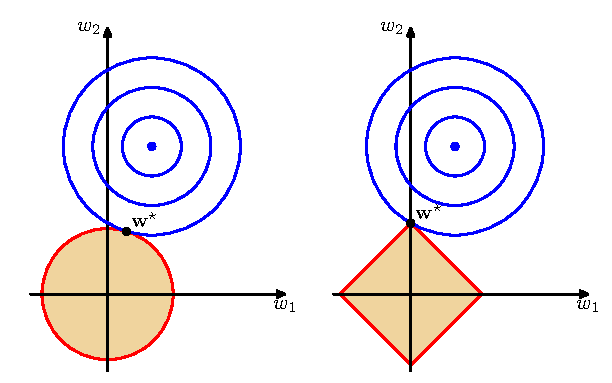
\includegraphics[width=0.75\textwidth]{reg.pdf}}
  \caption{Regularization as constrained optimization: the above shows the contour plots of a quadratic objective, and $L^2,L^1$ regularizations, respectively, as constraints constructed by weighing the objective against the shape of the regularizer's ball. Image from Bishop's Pattern Recognition and Machine Learning, Chapter 3, page 146.}
\label{fig:reg}
\end{figure}
\\\\
\noindent
\textbf{Proximal Regularization}. Similar to weight decay, but $\Omega(\vtheta)=\alpha\norm{\vw}_1$. Assuming a (convex) diagonal Hessian approximation to $J(\vtheta)$ (more strict than above), the $i$-th component solution is pulled down to
$$w_i=\begin{cases}
\pa{\abs{w_i}-\frac{\alpha}{H_{i,i}}}\sgn w_i  & H_{i,i}>0, \abs{w_i}>\frac{\alpha}{H_{i,i}}\\
  0 & \text{otherwise}
\end{cases}$$
$L^1$ regularization is equivalent to Bayesian MAP if weights have $\Laplace(0, \alpha^{-1})$ prior.
\\\\
\noindent
\textbf{Dataset Augmentation and Manifold Learning}. Modify supervised pairs $(\vx, y)$ to include $(T(\vx), y)$ where $T$ is a transformation we expect the classifier to be invariant to. Noise injection into inputs, too can be a form of dataset augmentation. An automatic technique for doing this is tangent propagation (\nurl{https://papers.nips.cc/paper/4409-the-manifold-tangent-classifier}{Rifai et al 2011}), which adds a penalty if the output is sensitive to changes along learned manifold vectors $\vv_i$: $\Omega(f)=\sum_i\pa{\vv_i^\top\nabla f)^2}$.
\\\\
\noindent
\textbf{Noise Robustness} (\nurl{https://papers.nips.cc/paper/4329-practical-variational-inference-for-neural-networks}{Graves 2011}). Inject noise into weights during training, forcing learned weights to be robust to small variations.
\\\\
\noindent
\textbf{Early Stopping}. Stop training if validation increases; even if training is unconverged. If validation set is large, you miss out on a lot of data. More complicated algorithms are necessary to find an applicable early stopping time when re-training to include validation set (see \nurl{http://www.deeplearningbook.org/contents/regularization.html}{Goodfellow's DL book}, Algorithm 7.3). Early stopping is similar to $L^2$ regularization, and for quadratic loss it is just that (Fig.~\ref{fig:earlystop}).
\begin{figure}[!h]
\centering
{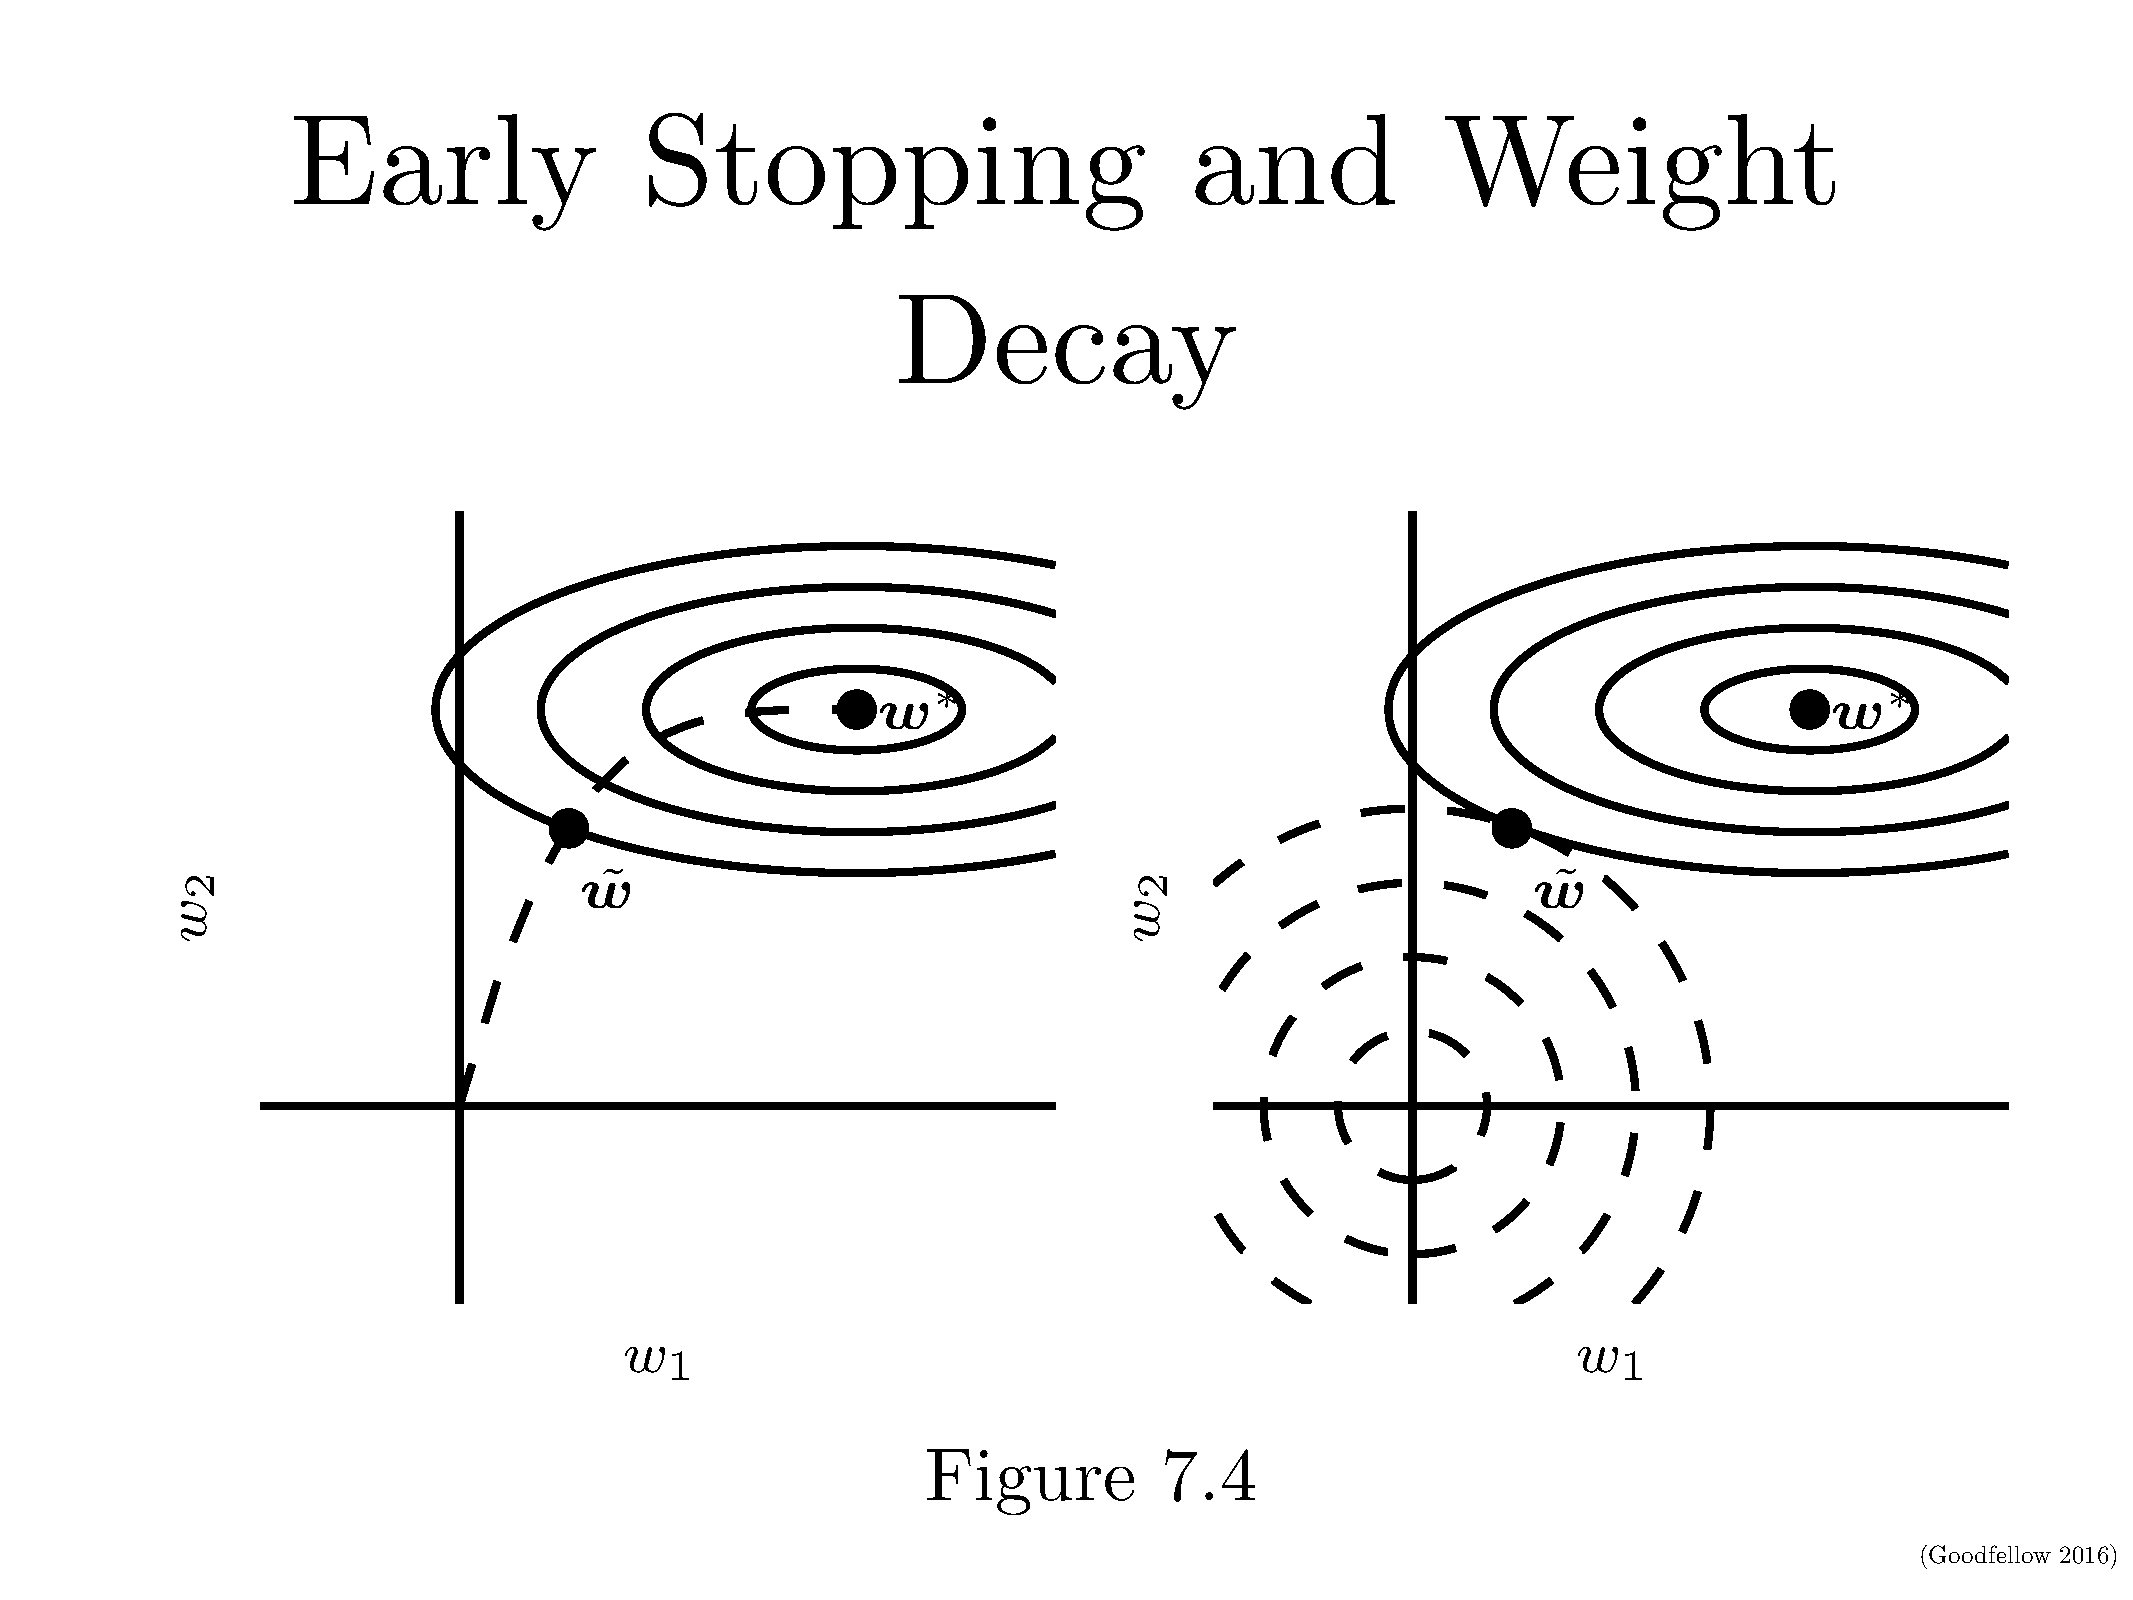
\includegraphics[width=0.75\textwidth]{early-stop.pdf}}
  \caption{From Dr. Goodfellow's DL book lecture, Chapter 7.}
\label{fig:earlystop}
\end{figure}
\\\\
\noindent
\textbf{Parameter Sharing}. Reuse part of a network for another task, encoding prior knowledge that the feature maps must be the same between two tasks. CNNs, below, are a form of parameter sharing, since the linear matrix $W$ is restricted to a convolution transform.
\\\\
\noindent
\textbf{Ensemble Methods}. Bagging uses votes of several models: $k$ uncorrelated models will tend to have $\nicefrac{1}{k}$-th generalization error when bagged. Training data can be resampled to create more uncorrelated models.
\\\\
\noindent
\textbf{Dropout} (\nurl{https://arxiv.org/abs/1207.0580}{Hinton et al 2012}, \nurl{http://proceedings.mlr.press/v28/wang13a.html}{Wang et al 2013}, \nurl{http://jmlr.org/papers/v15/srivastava14a.html}{Srivastava 2014}, \nurl{https://arxiv.org/abs/1506.02142}{Gal et al 2015}). Dropout is a cheap, practical approximation to averaging exponentially many models (exponential in the number of dropout layers). Dropout at a certain hidden or input layer wp $p$ drops an activation by setting it to zero during training and multiplying all activations (or the weights) by $p$ with no drops during testing (the weight scaling inference rule); theoretically this does not guarantee a proper output activation averaging, only individual hidden unit output expectation is preserved, but this works well in practice (Fig.~\ref{fig:dropout}). Weight scaling actually corresponds to taking a geometric means of the votes, and has been showed to work better than Monte Carlo sub-network averaging (which is intractable). First, this prevents feature co-adaptation: since a given activation might vanish at any time during training, the net is forced to learn those activations at each layer which independently contribute to the loss minimization task. Note that this conflicts with locality-focused tasks which rely on specific co-adaptations, like convolutional layers, but might be used at higher levels in CNNs to force the networks to identify more than one underlying feature for their classification (though lower levels can be locally co-adapted). Naive Bayes is an extreme form of dropout which demonstrates the co-adaptation avoidance.
\begin{figure}[!h]
\centering
{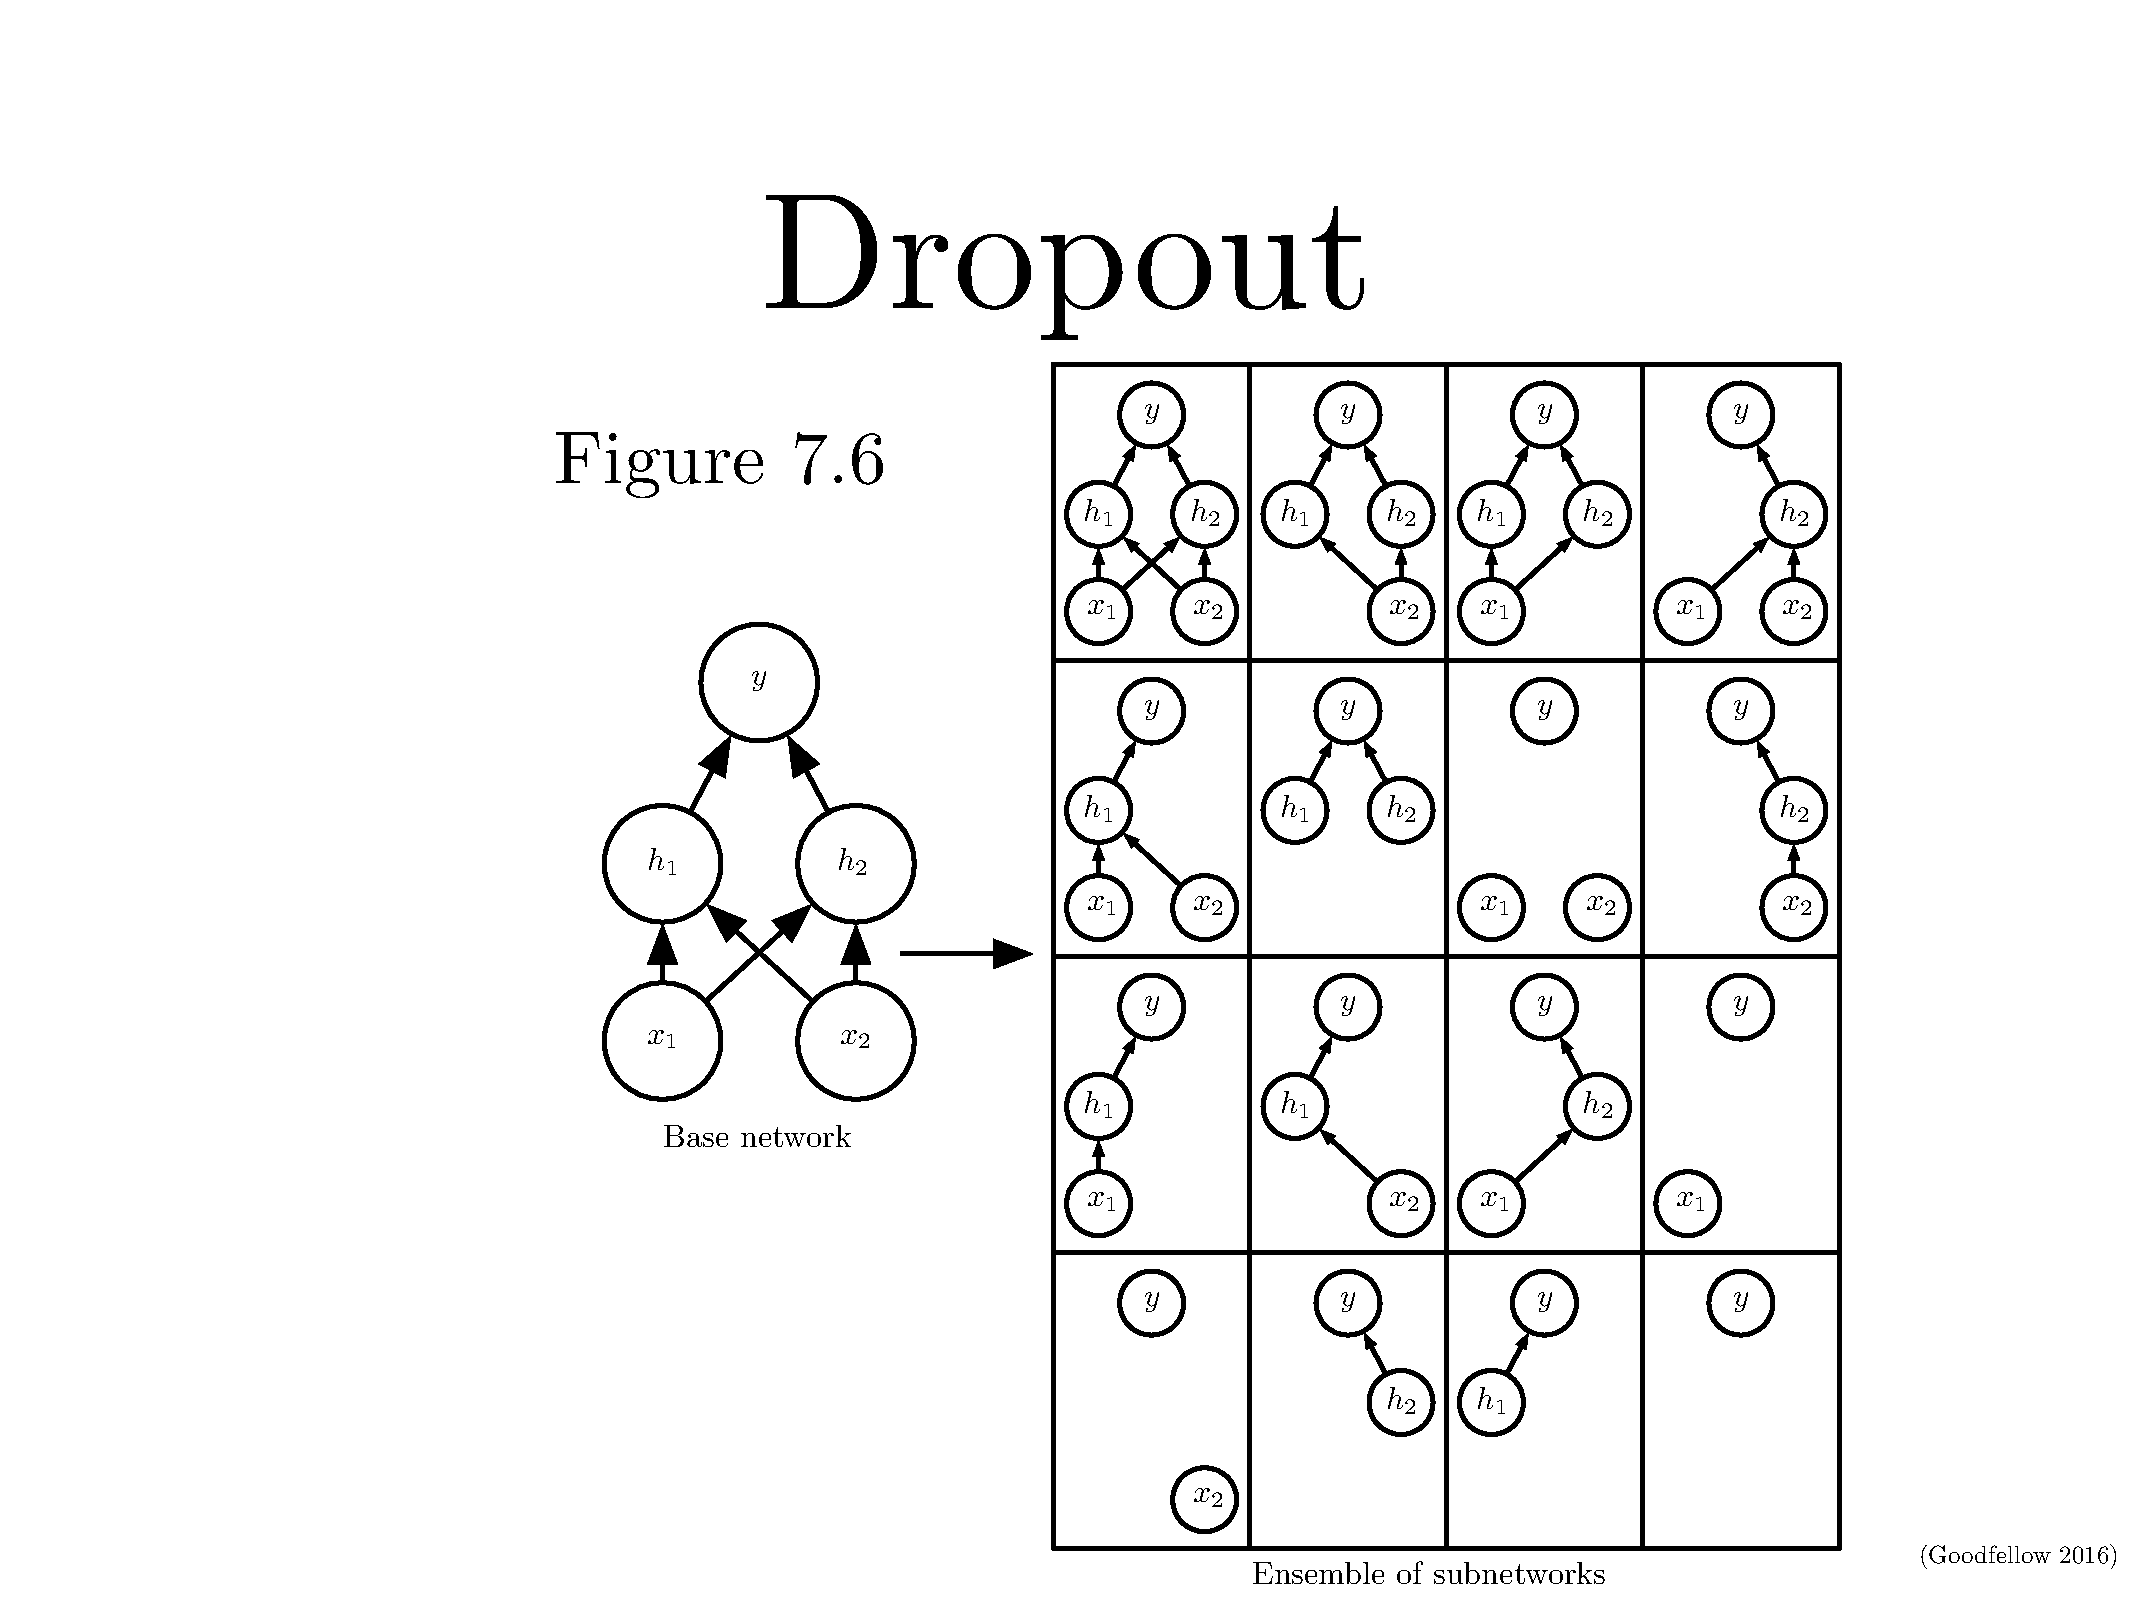
\includegraphics[width=0.75\textwidth]{dropout.pdf}}
  \caption{From Dr. Goodfellow's DL book lecture, Chapter 7.}
\label{fig:dropout}
\end{figure}
\\\\
\noindent
\textbf{Adversarial Training} (\nurl{https://arxiv.org/abs/1412.6572}{Goodfellow 2014}). Tiny changes in input can result in large differences in output, showing that the learned manifold for a classification category is too sensitive to perturbations in directions that it shouldn't be. Adversarial training forces nets to overcome this.

\section{Theory}

\noindent
\textbf{Universal Approximation Theorem}. A feed-forward network with a linear output layer, at least one hidden layer, and the logistic sigmoid activation can approximate any Borel measurable function and its derivatives, where they exist, arbitrarily well, given sufficient hidden units.
\\\\
\noindent
\textbf{Deep Rectifier Network Efficiency Theorem} (\nurl{https://arxiv.org/abs/1402.1869}{Mont\'{u}far et al 2014}). A deep rectifier network of constant width $w$, input dimension $i$ and depth $d$ may have up to $\Omega\pa{\pa{\nicefrac{w}{i}}^{di}i^i}$ distinct linear regions and a maxout network with $k$ filters per unit may have up to $\Omega(k^{i+l-1})$. Visually demonstrated in Figure~\ref{fig:montufar}.

\begin{figure}[!h]
\centering
{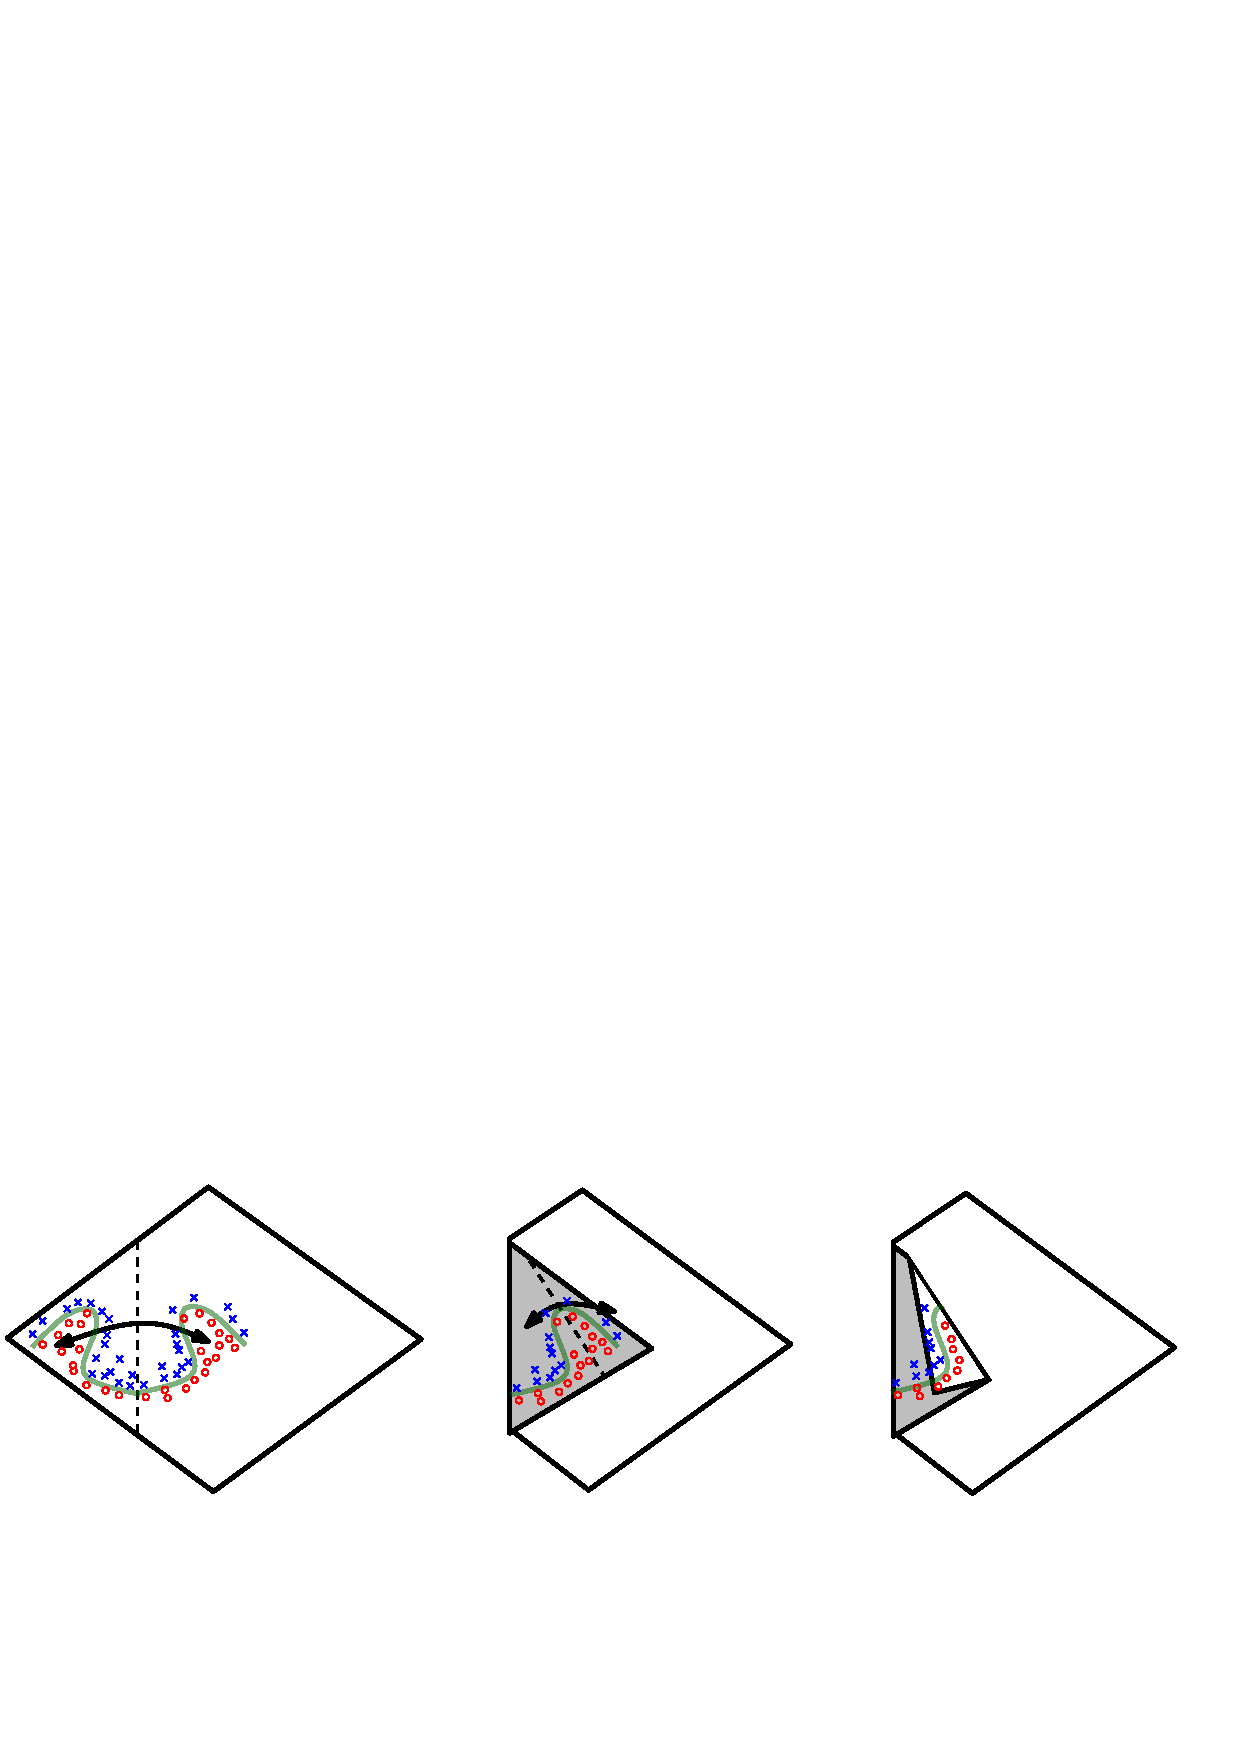
\includegraphics[width=\textwidth]{montufar2014.pdf}}
  \caption{Visual demonstration of how composing an absolute value rectifier, which in effect allows for a higher-level function to be mirrored over some hyperplane in the input space, can result in exponentially many different linear regions by relying on (learned) symmetry.}
\label{fig:montufar}
\end{figure}

\end{document}